\documentclass[JIP,draft]{ipsj}
\usepackage{graphicx}
\usepackage{amsmath}

\begin{document}
\title{Towards Cloud Bursting for Extreme Scale Supercomputers}

\begin{abstract}
Nowadays Supercomputers are widely used in scientifical computation, such as simulation and data analyse etc. 
Parallel programming are used to reduce execution time of complex problems, also fully utilizing computing resource of Supercomputers.
However, large serial applications will occupy computation nodes for a long time and causes some other applications which use numerous nodes to wait in a running queue, leads a low utilization of computing resource.
One solution is running virtual machine on 
In this paper, a comparision was made between a Public Cloud (AMAZON EC2) and a Supercomputer (TSUBAME) on Ethernet Performance and leading a 
\end{abstract}

\begin{keyword}
Supercomputer, Cloud, I/O Bursting Buffer Model
\end{keyword}

\maketitle

%1
\section{Introduction}
An increasing number of scientific applications are now running on Supercomputer for high performance computing nodes, large bandwidth and low latency interconnection environment, also a great number of processors for high scalability.
Data size need to be processed grows rapidly these days, which is known as Big Data, people perfer to use supercomputer to analyze Big Data for it supports high parallelism.

%Multi-user can use supercomputer at the same by using batch queue system which manage nodes and job submission.
However, when operating a supercomputer, there are some problems, high parallel application runs faster on Supercomputer for fully usage of computing resource, but a serial application will occupy computing nodes for a long time causing other application must wait.
Another problem is the power problem in summer, in order to reduce power comsumation, some nodes will be forced to be shutted down, reducing numbers of nodes will make the first problem more serous.
One solution is federating supercomputer with a public cloud, moving parts of job and computation to public cloud when there are not enough computing nodes available for user's request, which is known as cloud bursting.
Although cloud bursting is used by several companies and already have some sophisticated solution, since there are a significant performance gap between supercomputer nodes and cloud nodes, there will still be several problems when we try to ferderate a supercomputer with a public cloud.
The biggest problem will be data transfer throughput between two environment, supercomputers usual deal with Gigabyte or even Petabyte input and output of data, low I/O throughput will suffer supercomputer user. This paper focuses on methodology of increasing throughput when we do federation.

In order to increase data transfer throughput, we propose a I/O bursting buffer architecture that uses several nodes in each cloud as a I/O nodes to achieve high throughput concurrent data transferring, and a I/O bursting buffer model that uses to switch between I/O bursting buffer mode and direct connect mode.
This I/O bursting buffer architecture can be mainly used two situation, first in data I/O, the other one will be when there are some nodes need to migrate from a cloud to another cloud with snapshot, snapshots can be transferred without be stored to shared storage.
Since, I/O bursting buffer needs three times data transfer, sometimes direct transfer will achieve a higher throughput, I/O bursting buffer model using a evaluation throughput using I/O bursting buffer and without I/O bursting buffer to determine I/O bursting buffer mode or direct connection mode.
Also, public cloud usually charges for nodes usage, using I/O bursting buffer may reduce the computation time, but I/O nodes will be charged for money, we also provide a cost-based model, this model evaluate total cost with and without I/O nodes.

Our contribution can be summary as following:
\begin{itemize}
	\item An architecture of I/O bursting buffer for increasing data transfer throughput between two clouds.
	\item A throughput-based I/O bursting buffer model uses to switch between I/O bursting mode and direct connection mode in order to achieve a high data transfer when federating two clouds, and a cost-based I/O bursting buffer model uses to reduce the total cost.
	%\item 
	\item Evaluating I/O bursting buffer architecture and two models by using data obtained from several benchmarks from tsubame supercomputer and AMAZON EC2 public cloud.
\end{itemize}
%2
The remainder of this paper is orginized as follow:in section 2, the motivation and background of this study will be introduced, a overview of I/O bursting buffer Architecture including direct connection and I/O bursting buffer will be introduced in section 3, and the model used to switch between two modes will be described in section 4, a simulation result of our model %based on data obtained from several benchmark on TSUBAME V queue and AMAZON EC2 
will be shown in section 5, and finally, conclusion and related work will be seen in section 6.

\section{Motivation and Background}

%When people analyze large size of data, parallel programme is widely used in order to reduce computation time, especially when using supercomputer.
%However, it is usually difficult for a non-computer-scientist to write a parallel program, or re-write some existing applications into parallel version.
%Many serial applications are submitted to Supercomputer and occupy computing nodes for a long time, causing other applications which offer large number of nodes to wait for nodes, and leading a low utilization of computing resource.
%Consider following situation, there are 50 nodes available when a user submits a serial program using 1 node for 4 hours, after an hour a user try to run a program using 50 nodes, then he can't start his program until the first user finished his job.
%Such situation happens frequently when thousands and hundreds of users using one system at the same time and leading a low utilization of computing resource.
%One solution is running several virtual machines on a single physical machine for increasing utilization, which is used in TSUBAME Supercomputer, but sometime it still can't meet the request.
%For request not always reaches peak, it is not wise to increase nodes just for a temporary request peak.
%However even using virtual machines computing nodes still can't meet the request of users, for example, power problem will be critical in summer and nearly half of computing nodes have be shutted down to reduce electricity consumption in the case of TSUBAME Supercomputer.
Since the 
Facing these problems, one solution will be federate supercomputer with public cloud.
By using public cloud computing nodes just in request peak or when facing with power problem, people can save cost for buying new machines.
Of cause, there will be many challenges when Supercomputer federates with public cloud, such as security problems, using public cloud may cause research data opened to public, also connecting with Internet put Supercomputer under threats of hacker's attack.


%3
\section{I/O Bursting Buffer Overview}
An overview of I/O Burst Buffer architecture and two kinds of connection: direct connection and I/O bursting buffer are described in this section.
Although our goal here is to federate supercomputer with public cloud, since there are a great performance gap between normal supercomputer nodes and public cloud nodes and problem described above, here we consider about federating virtual machine nodes which running on supercomputer physical nodes with public cloud.
Since public clouds also run virtual machine on physical nodes, in the follow section, we treat the set of supercomputer's virtual machines as a cloud environment, also because only a few public IP address available in each cloud, I/O buffer nodes are required even in direct connection model.

%Reading operation describes operations when issues reading data from another cloud storage, and writing operation describes operation when issues writing data to another cloud storage

%Migration operation occurs when some nodes have to be shutted down in one cloud 
%all jobs running on these nodes have to be backed up by using snapshot, 

\subsection{Cloud Environment}
First each cloud is defined as follow:

%For security consideration and the fact that IPv4 addresses becomes rare,
All computing nodes are connected by large bandwidth and interconnection network, note network topology maybe different in each cloud, so topology is not specified here, interconnection network performance is measured by throughput.
There are a constant number of public IP addresses can be assigned to some computing nodes.
There is a shared storage for date sharing inside cloud, all computing nodes are connected with shared storage, also the filesystem of shared storage is not specified and performance is measured by throughput.


\subsection{I/O Bursting Buffer Architecture}

\begin{figure}[tb]
	\centering
%	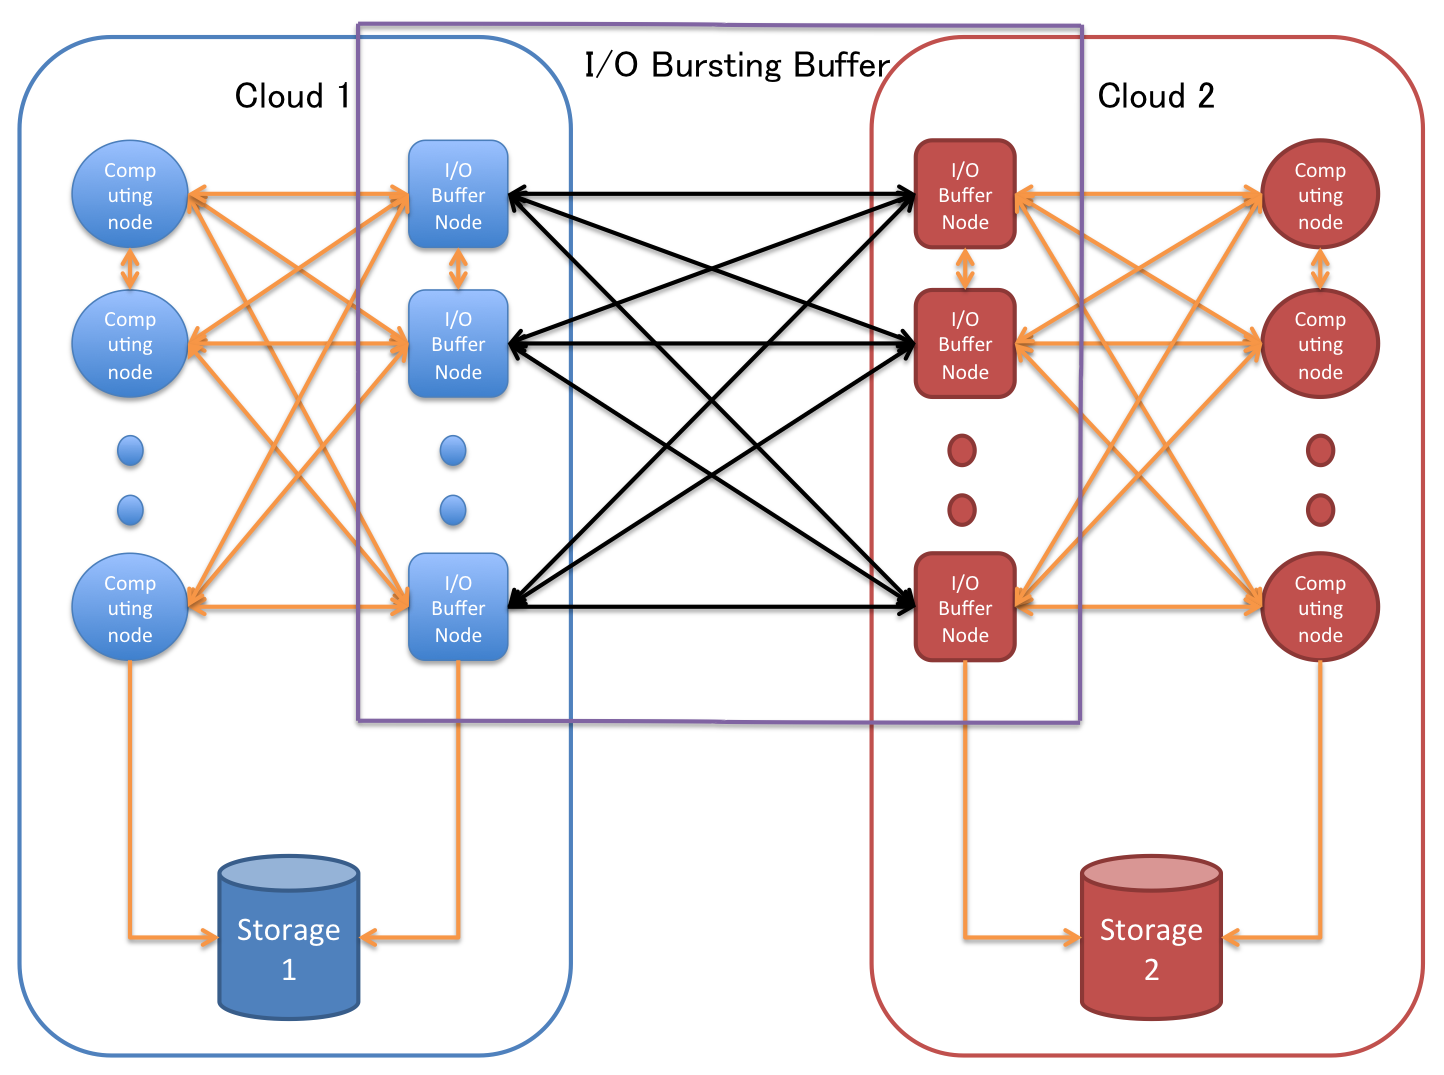
\includegraphics[width=6cm]{overview}
	\caption{overall illustrate of I/O Bursting Buffer Architecture}
	\label{overview}
\end{figure}

Fig.~\ref{overview} is the overall illustrate of I/O Bursting Buffer Model

There are two clouds here, cloud condition is defined above.

Arrows stand for network connection.
Orange arrows are innerconnection networks inside cloud, although two clouds used the same color for innerconnection networks, bandwidth can be different, also the topolopies are not specified and can be different in each cloud.
Black arrows are Internet connections, since there are a few amount of public IP addresses available, only I/O buffer nodes are connect to Internet, also the amount of available public IP address becomes the upper bound of the amount of I/O buffer nodes in each cloud. 
Although nodes with private IP address can use route or other net device to connect to Internet, but consider about security problem, also using route will reduce concurrent data transfer rate, here we assume all nodes in cloud only connect to local private network except I/O buffer nodes which connect to both local network and Internet.

Circles stand for computing nodes, which are used for standard computation.
Here we assume all computing nodes can communicate with each other, and also I/O buffer nodes and shared storage in the same cloud environment.
Squares are I/O buffer nodes, these nodes are used for data transfer between clouds, and are assigned with both public and private IP addresses.
I/O buffer nodes can use the same machine or VM as computing nodes, or can use network optimized nodes for larger throughput, but it is not required here.
Cylinders are shared storages, which are used to store data used by computing nodes, usually shared storage is consist of several nodes with a distributed filesystem and uses a better network, offers a large throughput.

%Since there is a big gap between cloud inside data transferring and accross two clouds in throughput, our goal is to fill the gap. 

For convenience, in the following section we assume data is stored in Cloud 1's shared storage, and computing nodes in Cloud 2 are used for computation. 

\subsubsection{Direct Connection}

\begin{figure}[tb]
	\centering
%	\includegraphics[width=8cm]{direct}
	\caption{direct access}
	\label{direct access}
\end{figure}

As Fig.~\ref{} shows, direct connection is a connection between I/O buffer nodes in cloud 2 and storage cloud 2 directly, only one side I/O buffer nodes are used in this model.
When computing nodes issue a read request, data firstly be splitted into number of I/O buffer nodes in cloud 2 pieces and assign one I/O buffer node one piece, then I/O buffer nodes start reading assigned data concurrently in order to fully utilize Internet bandwidth.
After reading finished, I/O buffer nodes send data to each computing node Simultaneously, there data will be restructure by using protocol described below.

Like reading, when computing nodes start to output data, first data will be buffered inside that nodes.
After output finished, data will be splitted into number of I/O buffer nodes in cloud 2 pieces, and assign one I/O node one piece, then data will be sent to all I/O buffer nodes concurrently.
When I/O buffer nodes received data, then they writing data back to storage in cloud 1.

\subsubsection{I/O Bursting Buffer}

\begin{figure}[tb]
	\centering
%	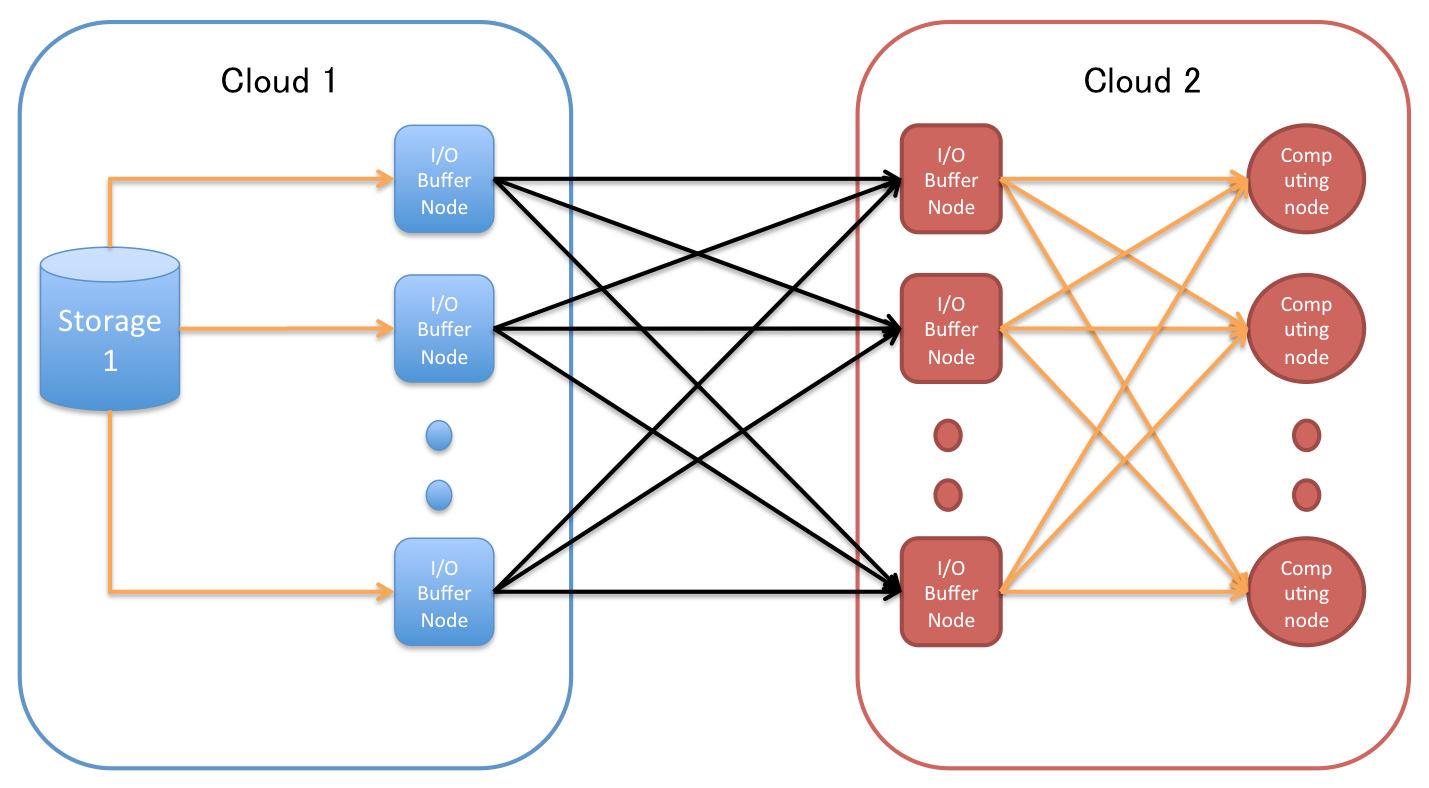
\includegraphics[width=8cm]{reading}
	\caption{data reading operation}
	\label{reading}
\end{figure}

\begin{figure}[tb]
	\centering
%	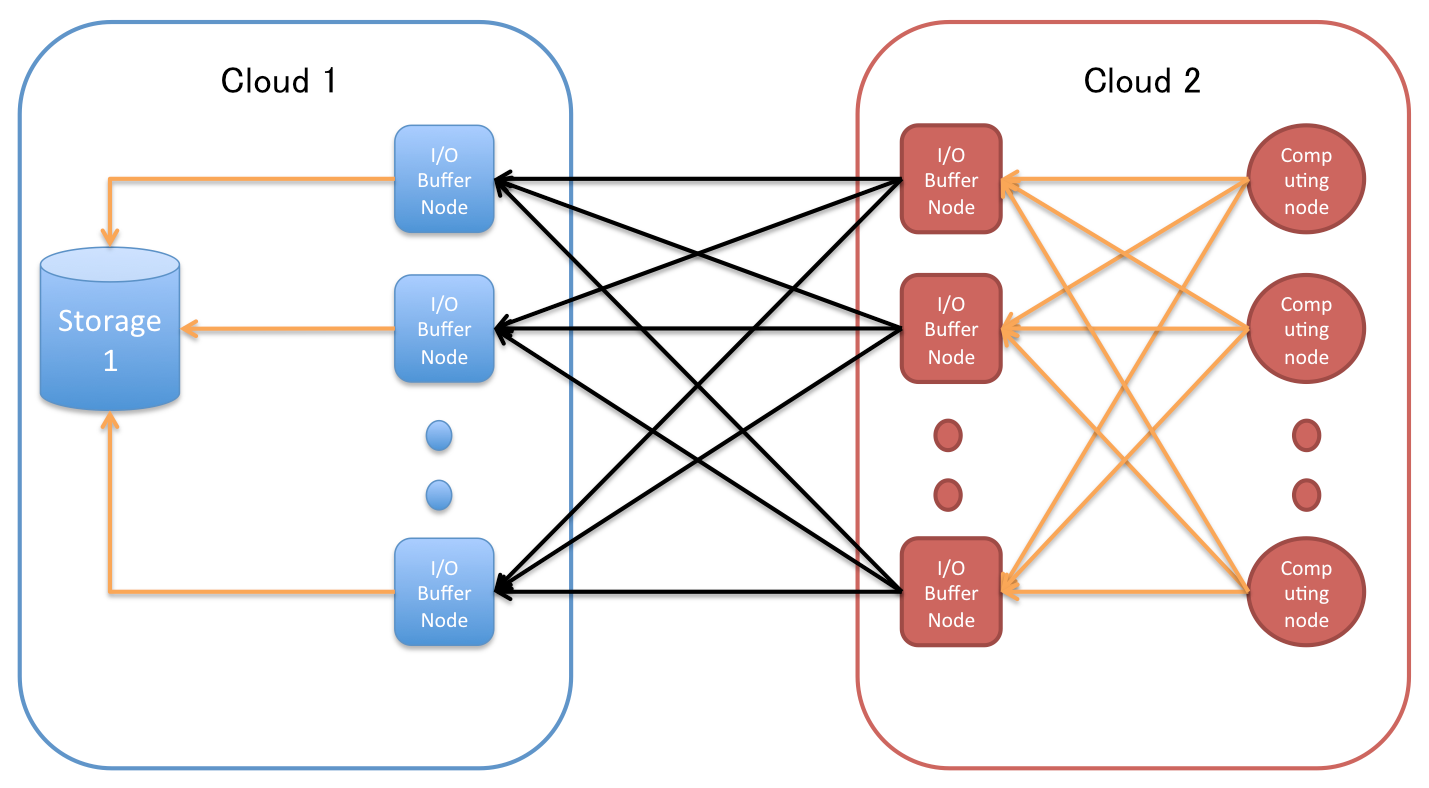
\includegraphics[width=8cm]{writing}
	\caption{data writing operation}
	\label{writing}
\end{figure}

I/O bursting buffer model may be used when throughput of direct connection between I/O buffer nodes and storage in different cloud is smaller then throughput between I/O buffer nodes, it is possible when storage is consist of few nodes, and direct connection will be 1-N connection, on the contrary, connection between I/O buffer nodes is N-N connection, has larger parallelism.

When computing nodes issue read request, first we check whether the file has been cached in I/O buffer nodes in cloud 1, if not, File will be splitted into the same number of I/O buffer nodes in cloud 1, and each I/O buffer node will be assigned a piece of split, then all I/O buffer nodes start reading assigned piece of data from shared storage simultaneously to fully utilize the bandwidth.% I/O buffer nodes use a main index to refer to the data position in global data.

After transferring data from shared storage finished, I/O buffer nodes in cloud 1 will connect with all I/O buffer nodes in cloud 2, then split data piece and into number of I/O buffer nodes in cloud 2,
%here a sub-index is used to refer to each piece's position, 
then transfer these pieces to I/O buffer nodes in cloud 2 concurrently in order to fully utilize Internet bandwidth.

When data transfer finished, I/O buffer nodes connect with all computation nodes which needs data, then transfer data to the corresponding position by using a index protocol described below, of cause all data transfer are done in parallel.

Data writing operation doing the opposite operation as reading operation.

When a computing node in cloud 2 issues data writing, output data will be first buffered by I/O server in that node.
After output finished, I/O server connects with all I/O buffer nodes in the same cloud, and split output data into the number of I/O buffer nodes, then send each piece of data to each I/O buffer nodes Simultaneously.

I/O buffer nodes then again split data into the number of I/O buffer nodes in cloud 1, like reading operation, here sub-index is used to refer to data position. and then start to transfer data concurrently. 

Then I/O buffer nodes write data to storage in cloud 1.

\subsubsection{Index Protocol}

\begin{figure}[tb]
	\centering
%	\includegraphics
	\caption{index protocol}
	\label{index protocol}
\end{figure}

As Fig.~\ref{index protocol} shows, two indexs are used in this protocol: main index and sub-index.
There are two phases of data splitting in both reading and writing operation, 

\section{I/O Bursting Buffer Model}

\begin{figure}[tb]
	\centering
%	\includegraphics
	\caption{definition}
	\label{definition}
\end{figure}

Throughput-based Model and Cost-based Model will be described in this section.
All definitions used are described in Fig.~\ref{definition}:

\begin{itemize}
	\item Numbers of computing nodes are $c_1,c_2$, and numbers of I/O buffer nodes are $n_1, n_2$ respectively.
	\item $D_1(n_2)$ is throughput when $n_2$ I/O nodes in cloud 1 connect to storage in cloud 2 directly, similar to $D_1(n_2)$, $D_2(n_1)$ refers to throughput when $n_1$ I/O nodes in cloud 2 connect to storage in cloud 1 directly, here we assume only I/O nodes in each cloud have Internet connection.
	\item Since overall Internet throughput is affected by number of nodes involved in connection. $I(n_1,n_2)$ is used to refer to Internet throughput using $n_1,n_2$ I/O buffer nodes respectively.
	\item For interconnection network throughput, although interconnection throughput is also affected by numbers of I/O nodes and computing nodes, numbers of users will running application on different number of computing nodes, it is difficult to compute each throughput, so here we use $E_1(n_1)$ to refer to limitation of maximum throughput of interconnection network in cloud 1 with $n_1$ I/O nodes, likely ,$E_2(n_2)$ is limitation of maximum throughput of interconnection network in cloud 2 with $n_2$ I/O nodes.
	\item $M_1(n_1),M_2(n_2)$ are throughput of connection between storage and $n_1$ I/O nodes in cloud 1 and ,storage and $n_2$ I/O nodes in cloud 2.
	\item Cost for standard node in cloud 1 is defined as $C_1\_Money(T)$ for $T$ time usage and cost for node in cloud 1 is $C_2\_Money(T)$ for $T$ time usage, and since I/O nodes may use a better network, here cost for I/O nodes is defined as $C_1\_High\_Money(T),C_2\_High\_Money(T)$ for $T$ time respectively.

\end{itemize}

\subsection{Throughput-based Model}
%There are many facts will affect throughput of Internet, so here a moniter is used to evaluate throughput between 
When I/O buffer nodes in cloud 2 connect to storage in cloud 1, there are two data transfers: computation nodes to I/O buffer nodes in cloud 2, I/O buffer nodes in cloud 2 to storage in cloud 1, so throughput will be:

\begin{equation}
	\text{throughput}_{\text{direct}}=\min\{D_1(n_2),E_2(n_2)\} \label{throughput1}
\end{equation}

In the case of using I/O buffer nodes in both cloud, there are three data transfers: computation nodes to I/O buffer nodes in cloud 2, I/O buffer nodes in cloud 2 to I/O buffer nodes in cloud 1, I/O buffer nodes in cloud 1 to storage in cloud 1, throughput will be:

\begin{equation}
	\text{throughput}_{\text{I/O buffer}}=\min\{M_1(n_1),I(n_1,n_2),E_2(n_2)\} \label{throughput2}
\end{equation}

In this throughput-based model, these two throughput are evaluated, and a switch is based on these two values:

\begin{equation}
	\begin{cases}
		\text{throughput}_{\text{direct}} \geq \text{throughput}_{\text{I/O buffer}} & \text{use direct connection}\\
		\text{throughput}_{\text{direct}} < \text{throughput}_{\text{I/O buffer}} & \text{use I/O buffer}
	\end{cases}
\end{equation}

\subsection{Cost-based Model}
In the case of cost-based model, we consider
using \ref{throughput1},and \ref{throughput2} total time for transferring unit size of data can be compute as:

\begin{equation}
	\begin{cases}
		T_1=\frac{1}{\min\{D_1(n_2),E_2(n_2)\}} & \text{direct connection}\\
		T_2=\frac{1}{\min\{M_1(n_1),I(n_1,n_2),E_2(n_2)\}} &\text{I/O buffer}
	\end{cases}
\end{equation}

here we compute cost by using $T_1,T_2$:
\begin{equation}
	\text{cost}_\text{direct}=c_2\times C_2\_Money(T_1)+n_2\times C_2\_High\_Money(T_1)
\end{equation}
\begin{align}
	\text{cost}_\text{I/O buffer}&=c_2\times C_2\_Money(T_2)\\\nonumber 
				     &+n_1\times C_1\_High\_Money(T_2)\\ \nonumber
				     &+n_2\times C_2\_High\_Money(T_2)
\end{align}


\subsection{Migration Model}
Since there are some condition that some supercomputer nodes must be shutted down, and jobs running on these nodes have to be migrate to another cloud. There are 
\begin{equation}
	Data	
\end{equation}
\section{Evaluation}
In this section, a simulation will be introduced based on data taking from several benchmarks on both TSUBAME and AMAZON EC2, 
\end{document}
